\documentclass[a4paper,10pt,article]{memoir}
\usepackage[utf8]{inputenc}
\usepackage[danish]{babel}
\usepackage{graphicx}
\usepackage{tikz}
% Hyppigt benyttede pakker

\usepackage{amsmath}
\usepackage{amssymb}
\usepackage{amsthm}
\usepackage{listings}
\usepackage{color}

% Farver

\definecolor{dkblue}{rgb}{0,0.1,0.5}
\definecolor{dkgreen}{rgb}{0,0.4,0}
\def\Red{\color{\ifdraft red\else black\fi}}
\def\Green{\color{\ifdraft green\else black\fi}}
\def\Blue{\color{\ifdraft blue\else black\fi}}
\def\Black{\color{black}}
\newcommand{\details}[1]{\iffull{\Blue#1}\fi}
\definecolor{linkColor}{rgb}{0,0,0.5}

% S�tninger mv.

\newtheorem{theorem}{Theorem}
\newtheorem{corollary}[theorem]{Corollary}
\newtheorem{lemma}[theorem]{Lemma}

\newtheorem{saetning}{S{\ae}tning}
\newtheorem{proposition}{Proposition}
\newtheorem{korollar}{Korollar}

\theoremstyle{definition}
\newtheorem{definition}{Definition}
\newtheorem{example}{Example}
\newtheorem{eksempel}{Eksempel}
\newtheorem{problem}[theorem]{Problem}

\newenvironment{bevis}{\begin{proof}[Bevis:]}{\end{proof}}

% Operationel semantik

\newcommand{\lag}{\langle}
\newcommand{\rag}{\rangle}
\newcommand{\setof}[2]{\ensuremath{\{ #1 \mid #2 \}}}
\newcommand{\set}[1]{\ensuremath{\{ #1 \}}}
\newcommand{\besk}[1]{\ensuremath{\lag #1 \rag}}
\newcommand{\ra}{\rightarrow}
\newcommand{\lra}{\longrightarrow}
\newcommand{\Ra}{\Rightarrow}

% M�ngdenotation

\newcommand{\pow}[1]{\mathcal{P}(#1)}
\newcommand{\Z}{\ensuremath{\mathbb{Z}}}
\newcommand{\Nat}{{\mathbb N}}
\newcommand{\Binary}{{\mathcal B}}
\newcommand{\defeq}{\stackrel{\mathrm{def}}{=}}

\newcommand{\dom}[1]{\mbox{dom}(#1)}
\newcommand{\ran}[1]{\mbox{ran}(#1)}

% Udsagnslogik

\newcommand{\logand}{\wedge}
\newcommand{\logor}{\vee}
\newcommand{\True}{\mathbf{t \! t}}

% Parenteser

\newcommand\lb {[\![}
\newcommand\rb{]\!]}
\newcommand{\sem}[1]{\lb #1 \rb}
\newcommand{\subst}[2]{\{  {}^{#1} / {}_{#1} \}}

\newenvironment{tuborg}{\left\{ \begin{array}{cc} }{\end{array} \right.}

% Flexible-length arrows (Copyright (C) 1995, Michael Rettelbach)

\makeatletter
\newdimen\lleng
\newdimen\bleng

\def\gummitrans#1{
  \setbox0=\hbox{$\stackrel{\,#1}{\mbox{}}$}
  \lleng=\wd0%
  \advance\lleng by 0.6em
  \;\raisebox{0ex}{$\stackrel{\,#1}{%
    \makebox[\lleng]{%
      \rule{0mm}{1ex}\mbox{}\leavevmode \xleaders
      \hbox {$\m@th \mkern -2.6mu \relbar \mkern -2.6mu$}\hfill\mbox{}}}$}%
  \hspace{-2.2ex}\rightarrow}

\def\Gummitrans#1{
  \setbox0=\hbox{$\stackrel{\,#1}{\mbox{}}$}
  \lleng=\wd0%
  \advance\lleng by 0.6em
  \;\raisebox{0ex}{$\stackrel{\,#1}{%
    \makebox[\lleng]{%
      \mbox{}\leavevmode \xleaders
      \hbox {$\m@th \mkern -2.6mu \Relbar \mkern -2.6mu$}\hfill\mbox{}}}$}%
  \hspace{-2.2ex}\Rightarrow}

\def\trans#1{\mathrel{\gummitrans{#1}}}
\def\Trans#1{\mathrel{\Gummitrans{#1}}}


% Bevisregler

% Med sidebetingelse

\newcommand{\condinfrule}[3]
           {\parbox{5.5cm}{$$ {\frac{#1}{#2}}{\qquad
            #3} \hfill  $$}}

% Uden sidebetingelse

\newcommand{\infrule}[2]
           {\parbox{4.5cm}{$$ \frac{#1}{#2}\hspace{.5cm}$$}}

% Regelnavn

\newcommand{\runa}[1]{\mbox{\textsc{(#1})}}

% Svar p� sp�rgsm�l

\newenvironment{svar}{\begin{quote}\noindent\textbf{Svar:}}{\end{quote}}


\title{Tavlenoter \\ \emph{Forelæsning om Endelige automater}}
\author{Rasmus Gadensgaard}
\date{5. februar 2013}

%%% BEGIN DOCUMENT
\begin{document}
\maketitle

\tableofcontents*

\chapter{Om kurset}

Eksamen:
\begin{itemize}
	\item Skriftlig
	\item Opgaver til hver kursusgang ligner eksamensopgaver
	\item Ingen hjælpemidler til eksamen pånær egne svar på tekstspørsmål "portfolio"
	\item I kurset skal man bedømme andres tekstspørgsmål for at få ens egne svar i sin portfolio.
	\item 80--85 \% bestod sidste år
\end{itemize}

Kurset omhandler matematiske teorier for programmers form og
adfærd. Målet med disse teorier er at kunne give beskrivelser, der er
uafhængige af en implementation. Det indeholder to dele:

\begin{description}
	\item[Syntaks] Der svarer på spørgsmålet: Hvad kan man skrive?
	\item[Semantik] Der svarer på spørgsmålet: Hvad sker der når et program bliver udført? 
\end{description}

Hver forelæsning introducerer nyt stof, så man skal læse \emph{efter}
hver forelæsning (men man må selvfølgelig også gerne læse stoffet inden).

\chapter{Indledning}

Denne forelæsning handler om

\begin{itemize}
\item Eksempel \{strenge, sprog osv.\}
\item Definition af DFA'er
\item Eksempler
\item Definition af accept, regulære sprog
\item Regulære operationer
\item Regulære sprog lukket under $\cup$ 
\item Gyser
\end{itemize}

\chapter{Grundlæggende begreber om sprog}

\begin{tabular}{| p{5cm} | p{5cm} |}
    \hline
    Definition & Eksempel \\ \hline
    Et \emph{alfabet} er en endelig mængde af \underline{tegn} & $B=\{0,1\}$ $A=\{a,b,c,d,e\}$ \\ \hline
    En \emph{streng} over alfabet $\Sigma$ er en endelig følge af tegn fra $\Sigma$ & $001 \in B^*$ , $aab \in A^*$ , $00a  \not \in  B*$  \\ \hline
    Mængden af alle strenge kalder vi $ \Sigma $* & \\ \hline
    Hvis $u,v \in \Sigma^{\ast}$ betegner uv \emph{kontatenationen} af $u$ og $v$ & $aab \in A^*$, $fed \in A^*$, $aabfed \in A^*$ \\ \hline
    Et sprog over $\Sigma$ er en delmængde af $\Sigma^{\ast}$, dvs. en
    mængde af strenge $\Sigma$ & $\emptyset$ er et sprog over $B$,
    $\{0,1\}$ er et sprog over $B$, $\{0,00,000,000, \ldots \}$ er et sprog over $B$, $\{aab, fete, acd\}$ \\ \hline
    \emph{Den tomme streng} kaldes $\varepsilon$ & \\ \hline
  \end{tabular}

\chapter{Endelige automater}

  
En endelig automat er en lille algoritme som afgør om en streng er en
del af et sprog. 

\begin{eksempel} \label{eks:e1}

I Figur \ref{fig:m1} ses et eksempel på en endelig automat. 

\begin{figure}
  \begin{center}
    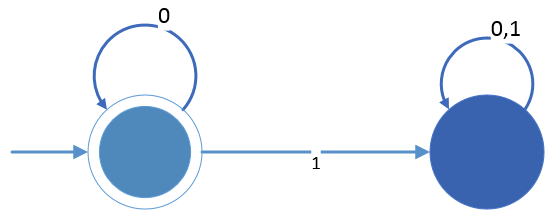
\includegraphics[width=60mm]{fig1.PNG} 
  \end{center}
\caption{En endelig automat $M_1$. Strengen $000$ accepteres af
  $M_1$. Derimod bliver strengen $001$ ikke accepteret.}
\label{fig:m1}
\end{figure}
\end{eksempel}

\begin{eksempel}
Betragt sproget
%
\[ L_1 = \setof{w \in \set{0,1}^*}{ w \text{ starter med 1, slutter
    med 0 }} \]
%
Figur \ref{fig:m2} viser dels en automat, der ikke genkender $L_1$, dels en automat, der genkender $L_1$.
\begin{figure}
\begin{center}
  \begin{tabular}{| c| c |}
    \hline
    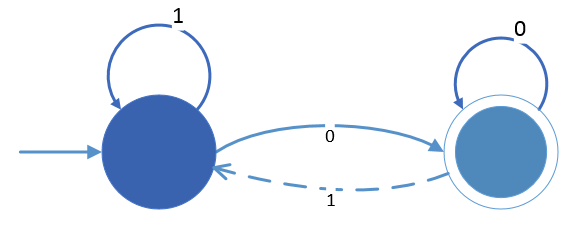
\includegraphics[width=60mm]{fig2.PNG} & 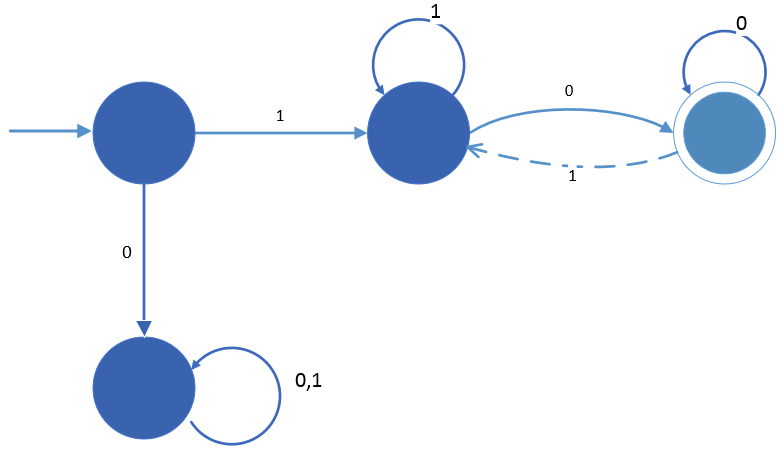
\includegraphics[width=60mm]{fig3.PNG} \\ \hline
     En ukorrekt automat (der ikke genkender $L_1$) & En korrekt
     automat for $L_1$ \\ 
    \hline
  \end{tabular}
\end{center}
\caption{To endelige automater}
\label{fig:m2}
\end{figure}

\end{eksempel}

  \section{Definition af endelig automat}
  
\begin{definition}
En endelig automat $M$ er en 5-tupel
%
\[ (Q,\Sigma,q_0,\delta,F)  \]
%
%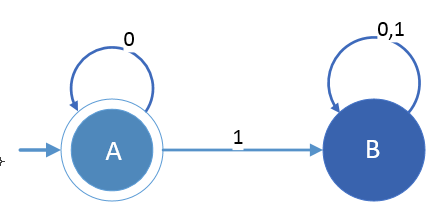
\includegraphics[width=60mm]{fig4.PNG}
hvor
\begin{align*}
Q \text{ er en endelig mængde af tilstande} \\
\Sigma \text{ er et endeligt alfabet} \\
q_0: \text{Startilstand, } q_0 \in Q \\
\delta: \text{Overføringsfunktion, } \delta:  Q \times \Sigma \ra Q \\
F: \text{Mængde af accepttilstande}, F \subseteq Q
\end{align*}
\end{definition}

\begin{eksempel}
Betragt igen automaten fra Eksempel \ref{eks:e1}. Vi har 
\begin{align*}
Q & = \{A,B\} \\
\Sigma & = \{0,1\} \\
q_0 & = A \\
F & = \{A\} 
\end{align*}

og overføringsfunktionen kan skrives op i tabelform som

\begin{center}
  \begin{tabular}{| l | c | c |}
    \hline
       & A & B \\ \hline
     0 & A & B \\ \hline
     1 & B & B \\
    \hline
  \end{tabular}
\end{center}
\end{eksempel}

\begin{definition}[Accept af streng]
Lad \[ A = (Q,\Sigma,\delta,q_0,F)  \]
være en DFA og lad
\[ w \in \Sigma^{\ast}, w=a_1 \ldots a_k  \]

$A$ \emph{accepterer} $w$ hvis $A$ ved at læse $w$ kan besøge
tilstande $r_0, ...., r_k$ så $r_k \in F$, dvs. der skal findes en
sådan følge af tilstande som opfylder at

\begin{itemize}
	\item $r_0$ = $q_0$
	\item for alle $0 \leq i \leq k$ har vi at $\delta(r_i, a_i)=r_i+1$
	\item $r_k \in F$ 
\end{itemize}

\end{definition}



\begin{definition}[Sproget genkendt af en automat]
 Sproget \emph{genkendt} af en DFA $A$ er givet ved \[ L(A) = \setof{w
   \in \Sigma^{\ast}}{A \text{ accepterer } w}  \]
\end{definition}



\begin{definition}[Regulært sprog]
 Et sprog kaldes regulært hvis det genkendes af en DFA
\end{definition}


\chapter{De regulære operationer}

De regulære operationer er 3 operationer, der kan anvendes til at
bygge sprog med.

Lad $L_1$, $L_2$ være sprog. Så er:
%
\begin{align*}
L_1 \cup L_2 & = \setof{x}{x \in L_1 \text{ eller } x \in L_2}  &
\text{(Foreningsmængde)} \\
L_1 \circ L_2 & = \setof{x}{\text{Der findes } u,v \text{ så } x=uv } &
\text{(Konkatenation)} 
\end{align*}

Lad $L$ være et sprog. Så er
%
\begin{align*}
L^* & = \setof{x_1 \ldots x_k}{k \geq 0, x_i \in L \text{ for alle } 0
  \leq i \leq k} & \text{(Kleene-stjerne)}
\end{align*}

Bemærk at vi ud fra definitionen får at $\varepsilon$ altid er element
i $L^{\ast}$.

Foreningsmængde og konkatenation kan imidlertid give et tomt sprog i
visse tilfælde. Vi har at 
%
\[ L_1 \cup L_2 = \emptyset \iff L_1=L_2=\emptyset \]  
%

\[ L_1 \circ L_2 = \emptyset \iff  L_1 = \emptyset
\text{ eller } L_2=\emptyset \]  
%
Vi har også at
%
\[ \emptyset^{\ast} = {\epsilon}  \]  
%
da $\varepsilon$ altid kommer med, når vi anvender
stjerne-operationen.

\chapter{De regulære sprog er lukket under $\cup$}

\begin{saetning}
Hvis $L_1$ og $L_2$ er regulære sprog, så er $L_1 \cup L_2$ også et
regulært sprog.
\end{saetning}

Ideen i beviset er at lave en automat, der genkender $L_1 \cup L_2$
ved at køre automater for $L_1$ og $L_2$ i parallel.

Figurerne \ref{fig:m11} og \ref{fig:m22} viser et eksempel på to
automater. Figur \ref{fig:m12} viser et

\begin{figure}
\begin{center}
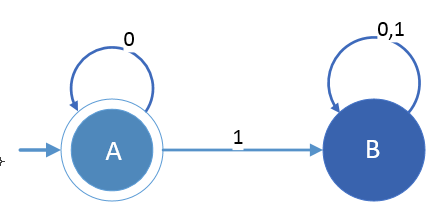
\includegraphics[width=60mm]{fig4.PNG}
\end{center}
\caption{Endelig automat $M_1$}
\label{fig:m11}
\end{figure}

\begin{figure}
\begin{center}
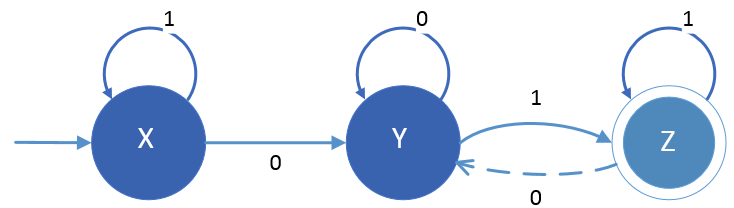
\includegraphics[width=60mm]{fig5.PNG}
\end{center}
\caption{Endelig automat $M_2$}
\label{fig:m22}
\end{figure}

\begin{figure}
\begin{center}
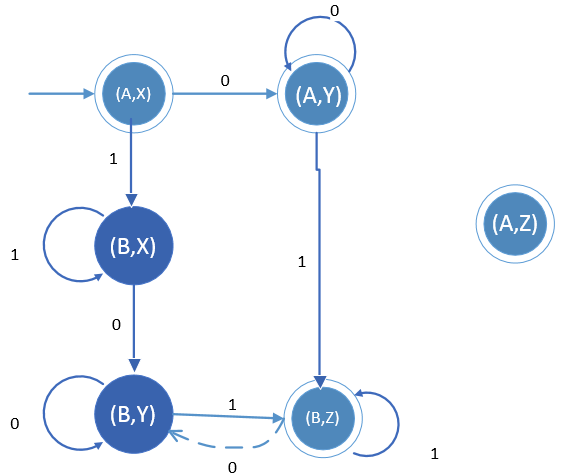
\includegraphics[width=60mm]{fig6.PNG}
\end{center}
\caption{Endelig automat, der kører $M_1$ og $M_2$ parallelt og
  genkender $L(M_1) \cup L(M_2)$}
\label{fig:m12}
\end{figure}

\begin{bevis}
Vi skal lave en DFS der genkender $L_1 \cup L_2$.
Vi ved at $L_1$ regulært, dvs. der findes en DFA $M_1$ så $L(M_1) =
L_1$ og at $L_2$ regulært dvs. der findes en DFA $M_2$ så $L(M_2) = L_2$.

Lad 
\begin{align*} M_1 & = (Q_1,\Sigma, q_1, \epsilon_1, F_1) \\
 M_2 & = (Q_2,\Sigma, q_2, \epsilon_2, F_2)
\end{align*}

Vores DFA for $L_1 \cup L_2$ er da
  
\begin{align*}
Q & = Q_1 \times Q_2 \\
q_0 & = (q_1, q_2) \\
F & = \setof{(p,q)}{p \in F_1 \text{ eller } q \in F_2}
\end{align*}
%
Overføringsfunktionen $\delta$ er givet ved 
%
\[ \delta((p,q),a) = (r_1, r_2) \text{ hvor }\delta_1(p,a)=r_1 \text{
  og } \delta_2(q,a)=r_2 \]
%
Denne \emph{produktkonstruktionen}.
\end{bevis}

Ud fra produktkonstruktionen er det meget nemt at vise at de regulære
sprog også er lukket under fællesmængde og under mængdedifferens. Vi
konstruerer en automat med samme slags tilstande og samme slags
overføringsfunktion; kun accepttilstandene er defineret anderledes.

\begin{itemize}
	\item Hvis $L_1, L_2$ regulære, så er $L_1 \cap L_2 $
          regulært. Her sætter vi
	\[ F = \setof{(p,q)}{p \in F_1 \text{ og } q \in F_2} \]
	\item Mængdedifferens er defineret ved \[ L_1 \setminus L_2 =
          \setof{x}{ x \in L_1, x \not \in L_2} \]
	Så har vi at hvis $L_1, L_2$ er regulære, så er $L_1 \setminus
        L_2$ regulært. Her sætter vi
	\[ F = \setof{(p,q)}{p \in F_1, q \in F_2 } \]
\end{itemize}

\chapter{Gyser}

\begin{itemize}
	\item Få styr på terminologien! -- det er vigtigt at kunne
        tale fagets sprog. Vi taler ikke om `sæt', `stadier',
        `transaktioner' osv. Og husk at `sprog' og `streng' ikke
        betyder det samme og ikke må anvendes i flæng!! \emph{Et sprog
          er en mængde af strenge.}
      \item En populær misforståelse blandt studerende er at den tomme
        streng skulle være med i ethvert sprog. Det gælder
        selvfølgelig ikke. Den tomme streng er ikke element i
        f.eks. $\set{ aab, abba}$. Personer, der holder af denne
        misforståelse, har ofte fejlhørt et udsagn om
        Kleene-stjerne. Det er korrekt at vi for ethvert sprog $L$ har
        at $\varepsilon \in L^{\ast}$.
\item En anden populær misforståelse blandt studerende er at
  konkatenation og kartesisk produkt `er det samme'. Men kontatenation
  er en operation, der bygger sprog (et sprog er en \emph{mængde af
    strenge}), mens kartesisk produkt bygger en mængde af ordnede
  par. Lad 
\begin{align*}
A & = \set{ aab, abba} \\
B & = \set{ bb, bbb, ba}
\end{align*}
%
Vi har
%
\[ A \circ B = \set{ aabbb, aabbbb, aabba, abbabb, abbabbb, abbaba} \]
som er en mængde af strenge, mens
%
\[ A \times B = \set{ (aab,bb), (aab,bbb), (aab, ba), (abba,bb),
  (abba,bbb), (abba,ba)} \]
%
Dette er to forskellige mængder.

Misforståelsen opstår formodentlig ofte, fordi nogle studerende har det med at
glemme at sætte parenteser om ordnede par. 
	\item Hvad betyder det at de regulære sprog er lukket under
          $\cup$? Nogle tror at det betyder at foreningsmængden af
          alle de regulære sprog er regulært. Men det gør det ikke.
	\item Mange glemmer, at sprog kan have uendeligt mange
          elementer. Et eksempel er sproget af alle strenge, der
          består af $0$ eller flere $0$er:
		\[ \{\epsilon, 0, 00, 000, ... \}) \]
	\item En populær misforståelse er at alle sprog er
          regulære. De, der holder af denne populære misforståelse, siger at det
          kan indses ved at betragte DFA'en $A$ på Figur
          \ref{fig:uha}.

\begin{figure}
\begin{center}
\begin{tikzpicture}[y=-1cm]

% objects at depth 50:
\draw[arrows=-to,black] (11.27008,4.3015) +(49:1.45283) arc (49:-220:1.45283);
\draw[black] (11.1125,6.82625) circle (1.68698cm);
\draw[black] (11.1125,6.82625) circle (1.24037cm);
\draw[arrows=-to,black] (7.9375,6.985) -- (9.36625,6.985);
\path (13.17625,3.81) node[text=black,anchor=base west] {\large{}$a \in \Sigma$};

\end{tikzpicture}%

\end{center}
\caption{En automat $A$, som mange fejlagtigt holder af}
\label{fig:uha}
\end{figure}
%
Det er klart at det for ethvert sprog $L$ gælder at denne automat
accepterer alle strenge fra $L$. Desværre accepterer den også alle
andre strenge! Vi har faktisk at $L(A)=\Sigma^{\ast} $.

En automat, der genkender et sprog $L$ skal acceptere de strenge, der
er elementer i $L$ \emph{og kun dem}.

\end{itemize}
\end{document}
